\section{Navigation}

Die Navigation zwischen den Aufgaben ist durch den Einsatz einer Tab-Basierten Navigation und Turbo blitzschnell.
Turbo ist eine JavaScript Bibliothek, welche einzelne Turbo-Frames über AJAX Requests austauschen kann. So sind keine Page-Reloads notwendig.

Die Tab-Navigation wurde in ein Turbo-Frame gesetzt. Die einzelnen Tabs sind Links, welche auf die anderen Aufgaben im Assessment zeigen.
Wird nun auf einen solchen Link geklickt, wird in der Response vom Backend nach einem Turbo-Frame gesucht, welches dieselbe ID hat. Der Inhalt
von diesem Frame wird dann ausgetauscht und der Rest der Seite bleibt gleich und behält auch ihren Zustand.

\begin{codebox}
\begin{minted}{ruby}
= turbo_frame_tag :task_nav do
  ul.nav.nav-tabs
    - @assessment.tasks.each do |task|
      li.nav-item
        = link_to task.title, [@assessment, task], class: 'nav-link'
\end{minted}
\end{codebox}

Für die Navigation zwischen den abgegebenen Lösungen wird ausserdem eine Pagination eingesetzt. Diese wurde mit dem \enquote{Pagy}
Gem implementiert.

\begin{codebox}
\begin{minted}{ruby}
- if @pagy.pages > 1
  == pagy_bootstrap_nav(@pagy)
\end{minted}
\end{codebox}

\begin{figure}[H]
  \centering
  
\includegraphics[width=\textwidth]{images/ui/pagination.png}
  \caption{\label{fig:pagt}Pagination mit dem \enquote{pagy} Gem}
\end{figure}

\section{Korrektur}

Die Assessment-Korrektur kann auf derselben Seite vorgenommen werden, auf der dieses auch gelöst wird.
Die abgegebenen Lösungen enthalten keine Namen oder E-Mail-Adressen und sind zufällig, nach deren Abgabezeitpunkt
sortiert. So wird eine unparteiische Korrektur ermöglicht.

Die hochgeladenen Dateien für jede Lösung werden einfach als Download-Links ausgegeben. 
So können diese für die Korrektur mit einem einzigen Klick heruntergeladen werden.

\begin{codebox}
\begin{minted}{ruby}
- uploads.each do |upload|
  = link_to rails_blob_path(upload, disposition: 'attachment')
\end{minted}
\end{codebox}

\begin{figure}[H]
  \centering
  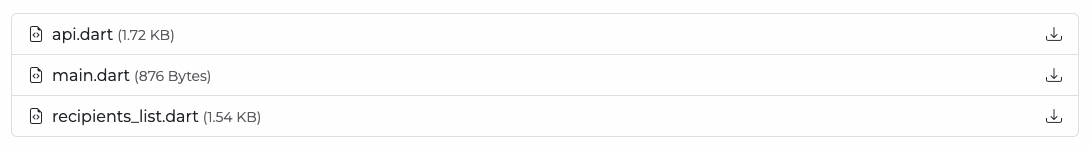
\includegraphics[width=\textwidth]{images/ui/download.png}
  \caption{\label{fig:download}Download-Links der abgegebenen Dateien}
\end{figure}

\newpage

Zu jedem dieser Lösungen können dann mehrere Korrektur-Kommentare abgegeben werden. Auch das Erfassen von Korrektur-Kommentaren wird durch den Einsatz von Turbo erleichtert,
indem diese real-time auf die Seite gestreamt werden.

Dazu gibt es nach jeder Lösung um die Kommentare eine Wrapper-Klasse mit einer bestimmten \emph{dom\_id}, welche automatisch
generiert wird.

\begin{codebox}
\begin{minted}{ruby}
div(id=dom_id(solution, :comments))
  = render solution.comments.with_all_rich_text
\end{minted}
\end{codebox}

Wird nun ein Kommentar erfasst, streamt das backend zum einen ein neues Formular an das Frontend und zum anderen
wird der neue Kommentar an die oben genannte Wrapper-Klasse \enquote{appended} und erscheint somit ohne Site-Reload direkt auf dem Bildschirm.

\begin{codebox}
\begin{minted}{ruby}
render turbo_stream: [
  turbo_stream.replace(comment, partial: 'comments/form', locals: { comment:, solution: @solution }),
  turbo_stream.append(dom_id(@solution, :comments), partial: 'comments/comment', locals: { comment: @comment })
]
\end{minted}
\end{codebox}
